\section{Introduction}

\par
(1) Keep the section 1 (context, problematic).


\vspace{8pt}
\par (2) Motivation: Why we choose this approach of automatically tuning the hyperparameter without modifying the choosen DR methods?

+ Easy to adapt to the existing DR methods. 

+ Towards AutoML (need citation) but can keep the explainability. Our method not only find the optimal visualization but also explain why it is.


\vspace{8pt} \par
(3) Add a small paragraph to introduce several visualization methods which are widely used in practice but hard to tune the (hyper)-hyperparameters:
tSNE~\cite{maaten2008tsne}, LargeVis~\cite{tang2016visualizing}, UMAP~\cite{mcinnes2018umap}.

\vspace{8pt} \par
(4) Our solution:

+ Constraint preserving score to measure the similarity preserving in the visualization. (TODO need to find the goal of our score, and say why it is worth to measure the similarity in the viz).

+ Bayesian Optimization (BayOpt) approach~\cite{mockus1978application, brochu2010tutorial} for hyperparameter tuning.

\vspace{8pt} \par
(5) Main contributions: 
TODO: Complete later.

To Discuss: What is exactly our goal: tune the hyperparameter (w.r.t. a score/metric) or to find the best visualization (w.r.t. to the evaluation of the real user for example)?

\vspace{8pt}
\par
(6) The target audiences:

+ The end-users who want to apply the visualization methods to their own data without caring about the complex algorithms and hyperparameters.
They can use our method as a blackbox hyperparameter tuning toolbox with an additional price of providing the labels or a partial of the labels for the dataset.
(Refer to the section analyzing the impact of the number of constraints).

+ The experts who want to analze the impact of the hyperparameters and to evaluate the quality of the visualization.
They can use our method as a transparent toolbox to understand the internal step in the optimization process thanks to BayOpt approach.



%%%%%%%%%%%%%%%%%%%%%%%%%%%%%%%%%%%%%%%%%%%%%%%%%%%%%%%%%%%%%%%%%%%
\section{Background and Related Work}

\subsection{Visualization Quality Metrics}
Keep the session 4.3

\subsection{Usage of Pairwise Constraints in Unsupervised Learning}
Keep the sections 3.2, 3.3.

\subsection{Choosing the Hyperparameters for DR Methods}
+ Automatic selection of perplexity for t-SNE, Cao and Wang~\cite{cao2017automatic}.

+ Modification of t-SNE that takes the labels to adjust the width of Gaussian neighborhoods instead of the manually selected perplexity.

+ Analyze the pros and cons of this method.

+ This method can be referred as a baseline to compare with our approach.

\subsection{Automatic Hyperparameter Tuning with Bayesian Optimization}

(1) Intro to BayOpt:

+ Refer to Mockus' serie of works on Bayesian method for seeking the extremum (Mockus1978, Mockus1982, Mockus1994).

+ Refer to the modern inroduction to BayOpt~\cite{brochu2010tutorial} with examples of its applications.


\vspace{8pt} \par
(2) Explain how BayOpt fits into our problem.

\vspace{8pt} \par
(3) Discuss: BayOpt can be applied to the BIC-based score~\cite{cao2017automatic}.
However this score has two disavantages:
(1) it is tied to the loss function of t-SNE.
(2) it works only with one hyperparameter (perplexity of t-SNE), and thus can not be generalized for other DR methods.
Our proposed method can do better.



%%%%%%%%%%%%%%%%%%%%%%%%%%%%%%%%%%%%%%%%%%%%%%%%%%%%%%%%%%%%%%%%%%%
\section{Constraint Preserving Score}

\subsection{Visual Definition of the Pairwise Constraints}
+ Keep the section 4.1

+ Explain that  we use the auto-generated pairwise constraints when having labels.

+ We can ask the user to label a small proportion of labels in order to construct the pairwise constraints, or the user can select the constraints manually.

\subsection{Quantify the Pairwise Constraints}
+ Keep the section 4.2 (first 3 paragraphs)

+ Add a sketch to illustrate the small distance of a similar link leads to large probability $q_{ij}$, thus a large score for must-link constraint. (the same for cannot-link constraint).

\subsection{Behaviour of Constraint Preserving Score}

+ Keep the section 4.2 (last paragraph)

Analyze the behaviour of the proposed score with respect to the global and local structure of the visualization as in~Fig.\ref{fig:score}.

\begin{figure}
\centering
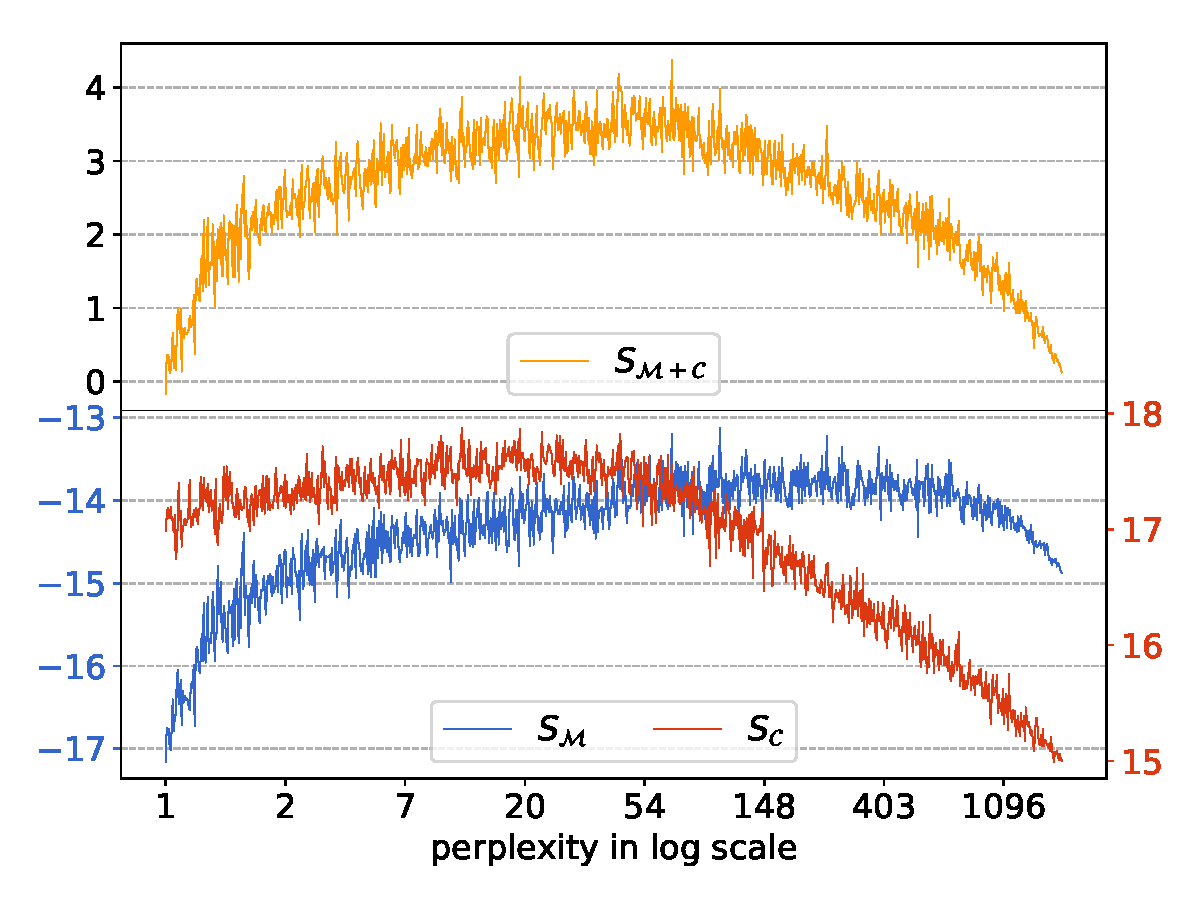
\includegraphics[scale=0.4]{s_scores_50.pdf}
\caption{Behaviour of the constraint-based score.}\label{fig:score}
\end{figure}



%%%%%%%%%%%%%%%%%%%%%%%%%%%%%%%%%%%%%%%%%%%%%%%%%%%%%%%%%%%%%%%%%%%
\section{Constraint-based Score as Target in Bayesian Optimization Approach}

+ Explain the internal step in BayOpt.
Can make use some figures Fig.~\ref{fig:bayopt5}, Fig.\ref{fig:bayopt10}.

\begin{figure}
\centering
\includegraphics[scale=0.25]{{ucb_kappa5_constraint1.0_DIGITS_step5}.png}
\caption{BayOpt after 5 steps.}\label{fig:bayopt5}
\end{figure}


\begin{figure}
\centering
\includegraphics[scale=0.25]{{ucb_kappa5_constraint1.0_DIGITS_step10}.png}
\caption{BayOpt after 10 steps.}\label{fig:bayopt10}
\end{figure}

+ Explain how the utility function are constructed and optimized, and answer why optimize the utility function (surrogate function), we can optimize at the same time the target function (the constraint-based score function).

+ Explain the exploitation-exploration trade-off in BayOpt (and estimate the number of times we need to try before reaching to the global maximum).

%+ Note about the nature of BayOpt that, it can work with any non-convex multi-modal objective function and it assures to find the global extremum.



%%%%%%%%%%%%%%%%%%%%%%%%%%%%%%%%%%%%%%%%%%%%%%%%%%%%%%%%%%%%%%%%%%%
\section{Experimental Results}

Present the dataset, the used pairwise constraint, the workflow as in the section 5.1, 5.2.

To present and analyze the results, we can present following points (but we still miss the evaluation).

(1) Optimal hyperparameters found by BayOpt w.r.t the constraint-based score:

+ BayOpt method for finding \verb|perplexity| param for t-SNE. (Case of 1 param to tune with t-SNE, Fig.~\ref{fig:tsne1}) (Done)
\begin{figure*}
\centering
\includegraphics[width=.6\textwidth]{{tSNE_ucb_kappa5_constraint1.0_DIGITS_step15}.png}
\caption{BayOpt with t-SNE with 1 param.}\label{fig:tsne1}
\end{figure*}

+ Add experiment with LargeVis. (TODO)

+ \st{BayOpt for finding n-neighbors param for UMAP. (Case of 1 param to tune with UMAP) (Done) } %Fig.~\ref{fig:umap1})
%% \begin{figure*}
%% \centering
%% \includegraphics[width=.6\textwidth]{{UMAP_ucb_kappa5_constraint1.0_DIGITS_step15}.png}
%% \caption{BayOpt with UMAP with 1 param.}\label{fig:umap1}
%% \end{figure*}

+ BayOpt for finding \verb|n_neighbors| and \verb|min_dist| params for UMAP. (Case of 2 params to tune with UMAP, Fig.~\ref{fig:umap2}) (Plan to do)
\begin{figure*}
\centering
\includegraphics[width=0.6\textwidth]{{demo_bayopt_2params}.png}
\caption{TODO: Produce a figure similar to this one with 2 params of umap.}\label{fig:umap2}
\end{figure*}

\vspace{8pt} \par
(2) Visualization of the violated constraints. (Doing, a draft version looks like
Fig.\ref{fig:viz-score})
We can analyze the explainability of the score / the visual assessment of the quality.

\begin{figure}
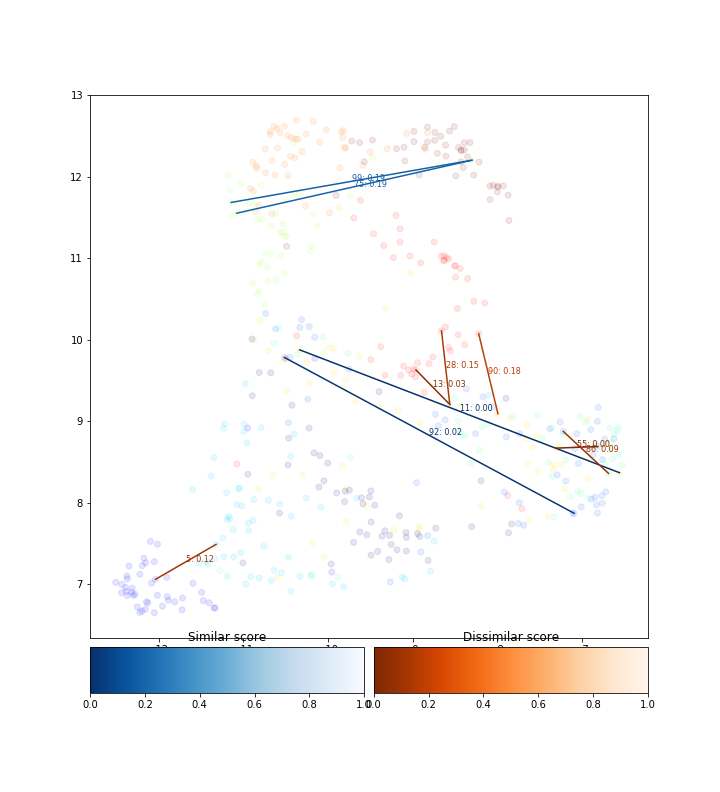
\includegraphics[scale=0.3]{umap_vis_score.png}
\caption{TODO Visualize the constraint score (of the violated links).}\label{fig:viz-score}
\end{figure}


\vspace{9pt} \par
(3) Analyse the characteristics of the constraint-based score.

+ Keep the section 6.2:

\hspace{10pt }- Must-link score agrees with CCA score (Fig~\ref{fig:sml}).
\begin{figure}
\centering
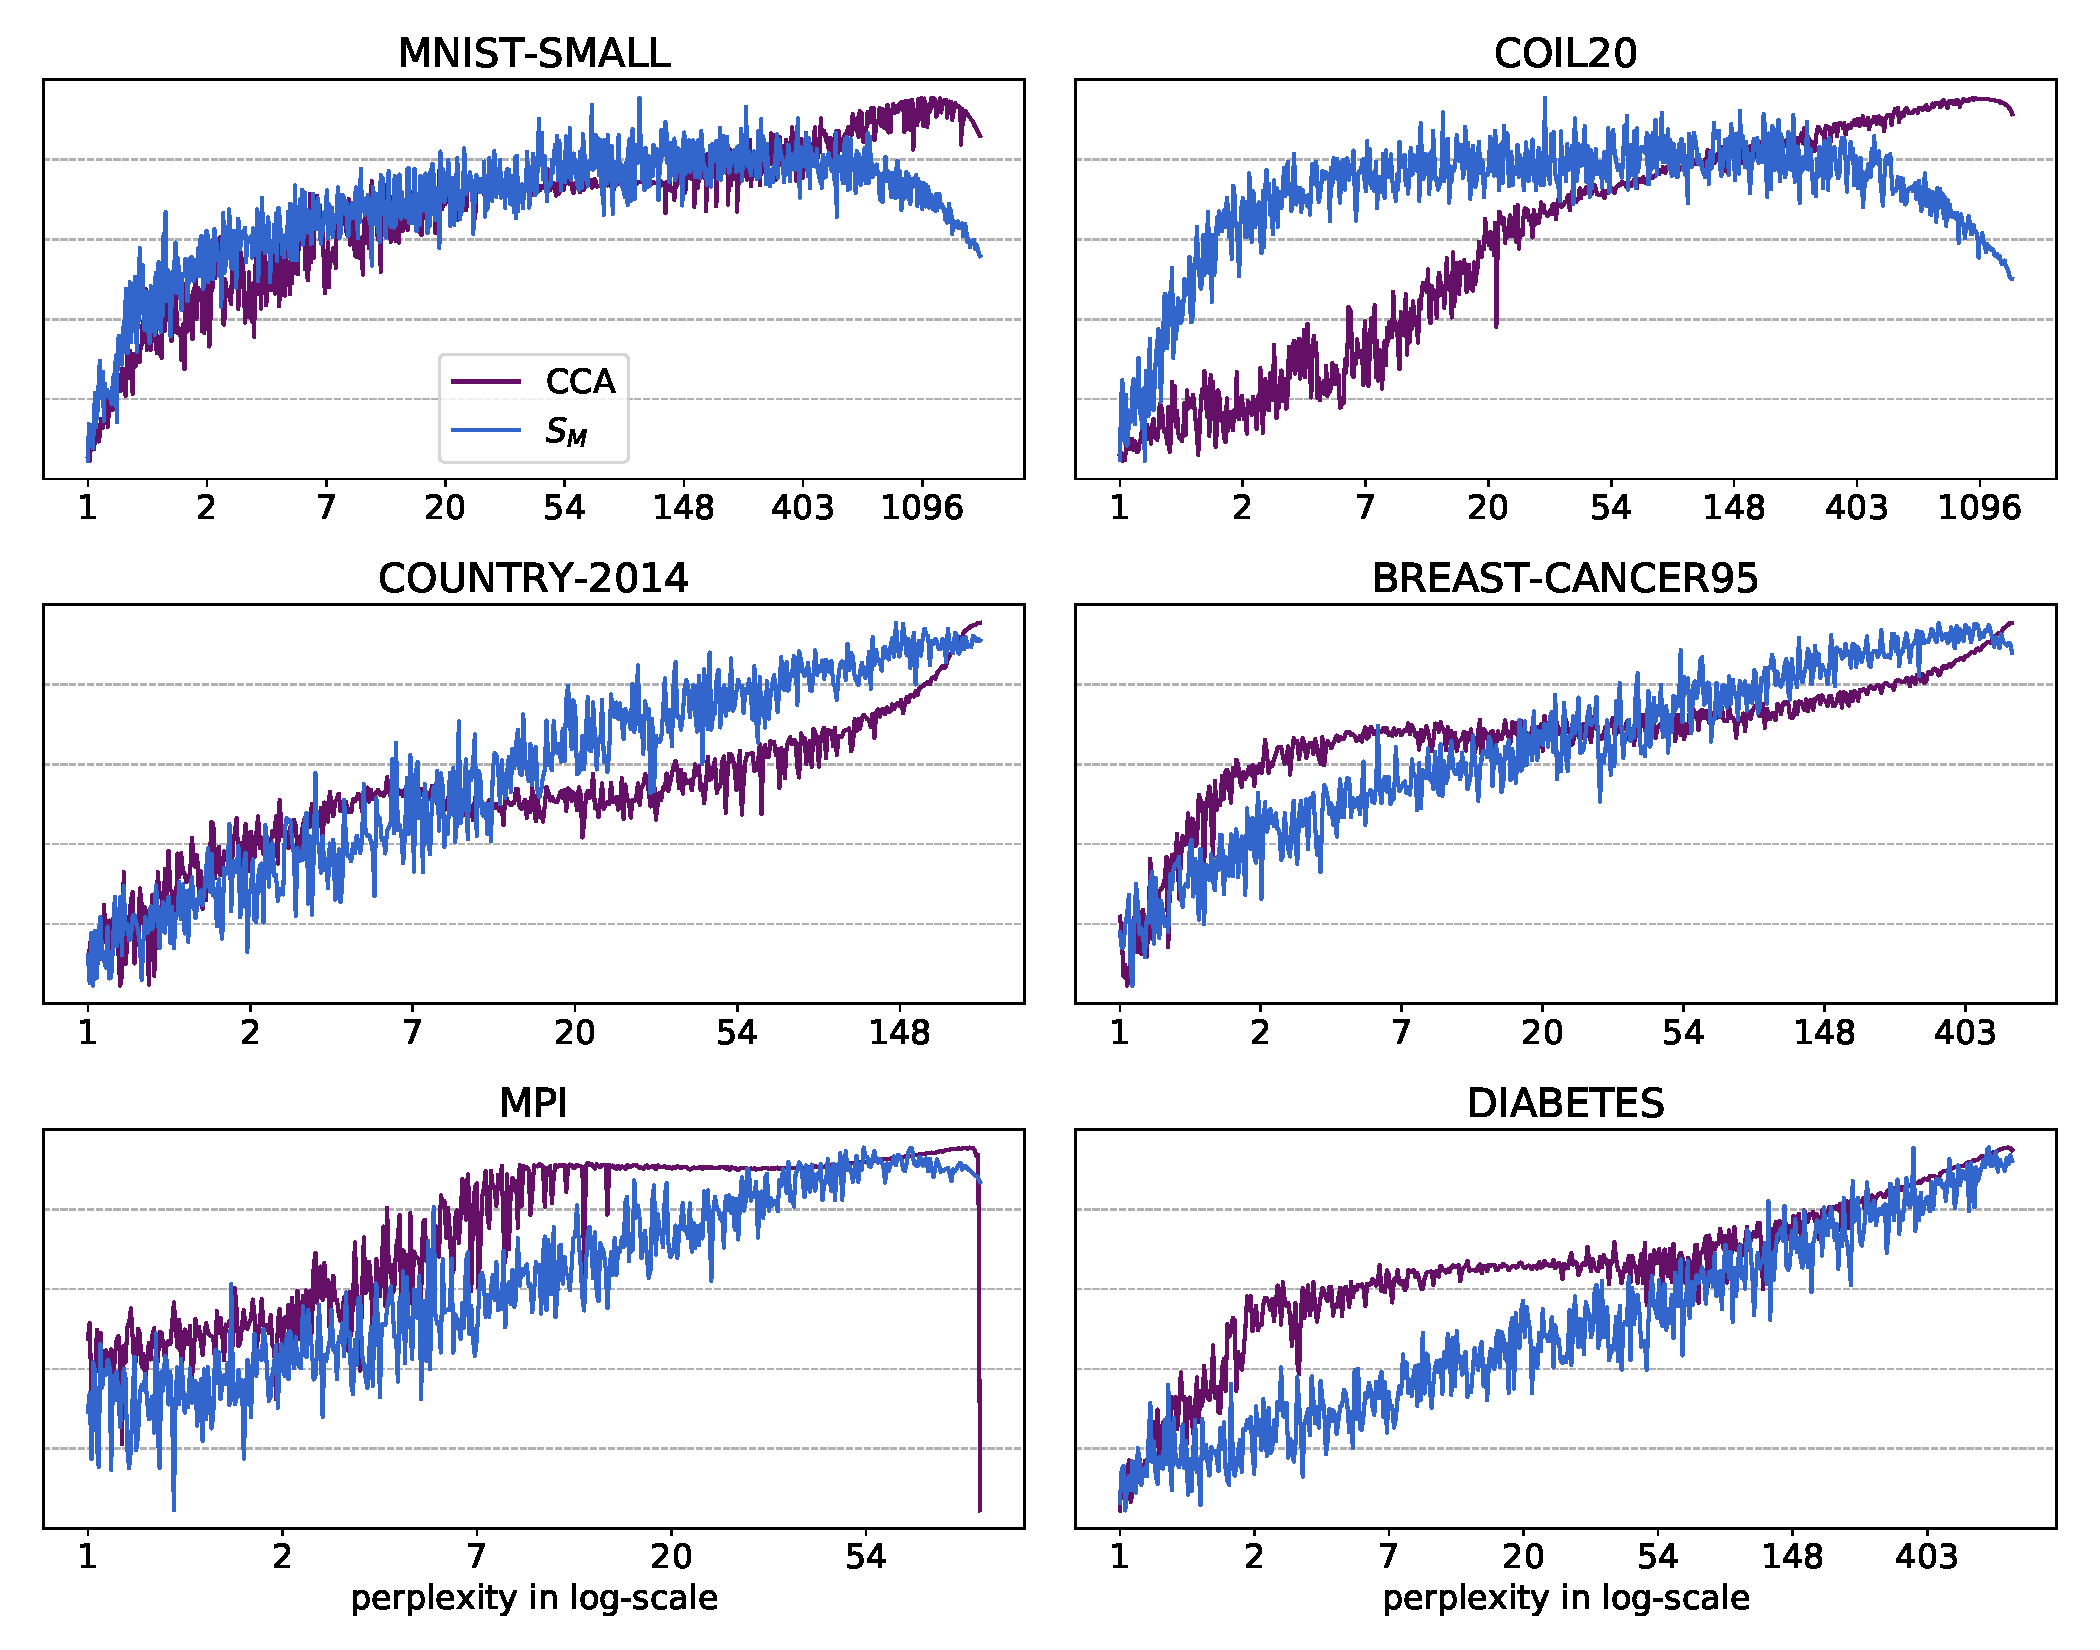
\includegraphics[scale=0.25]{sml_cca_50.pdf}
\caption{Must-link score agrees with CCA score.}\label{fig:sml}
\end{figure}

\hspace{10pt }- Cannot-link score agrees with BIC-based score (Fig.~\ref{fig:scl}).
\begin{figure}
\centering
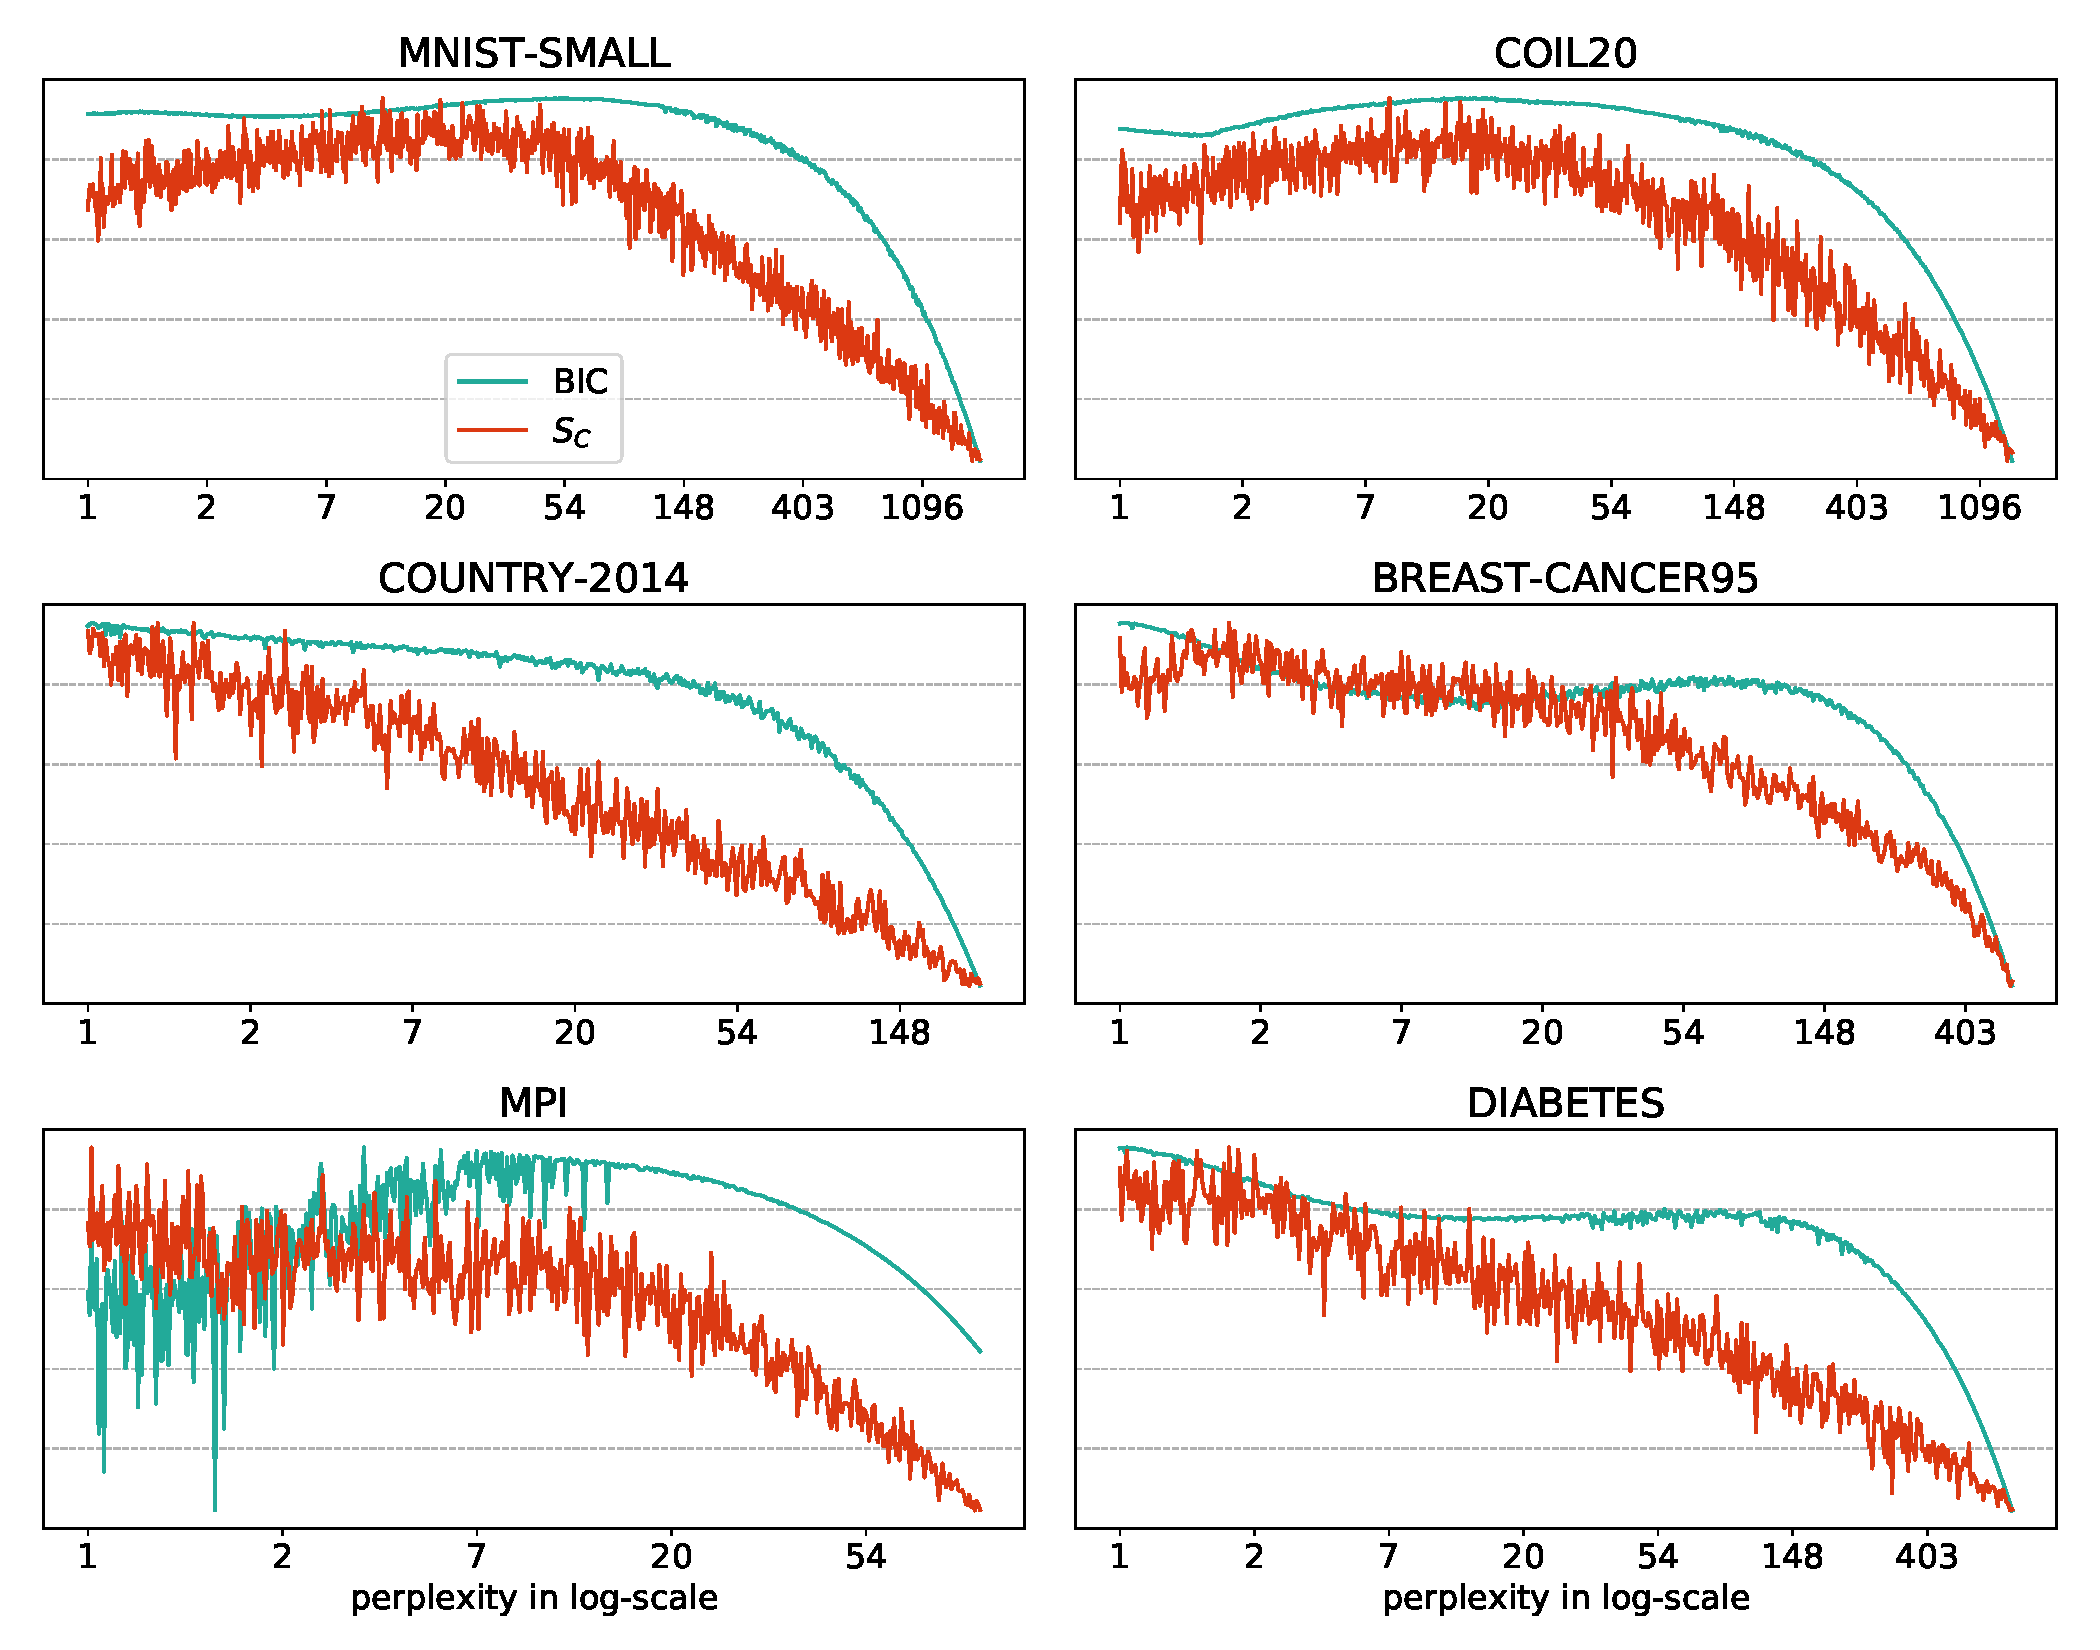
\includegraphics[scale=0.25]{scl_bic_50.pdf}
\caption{Cannot-link score agrees with BIC-based score.}\label{fig:scl}
\end{figure}

\hspace{10pt }- ML+CL agrees with AUC\_RNX score (Fig.~\ref{fig:sall}).
\begin{figure}
\centering
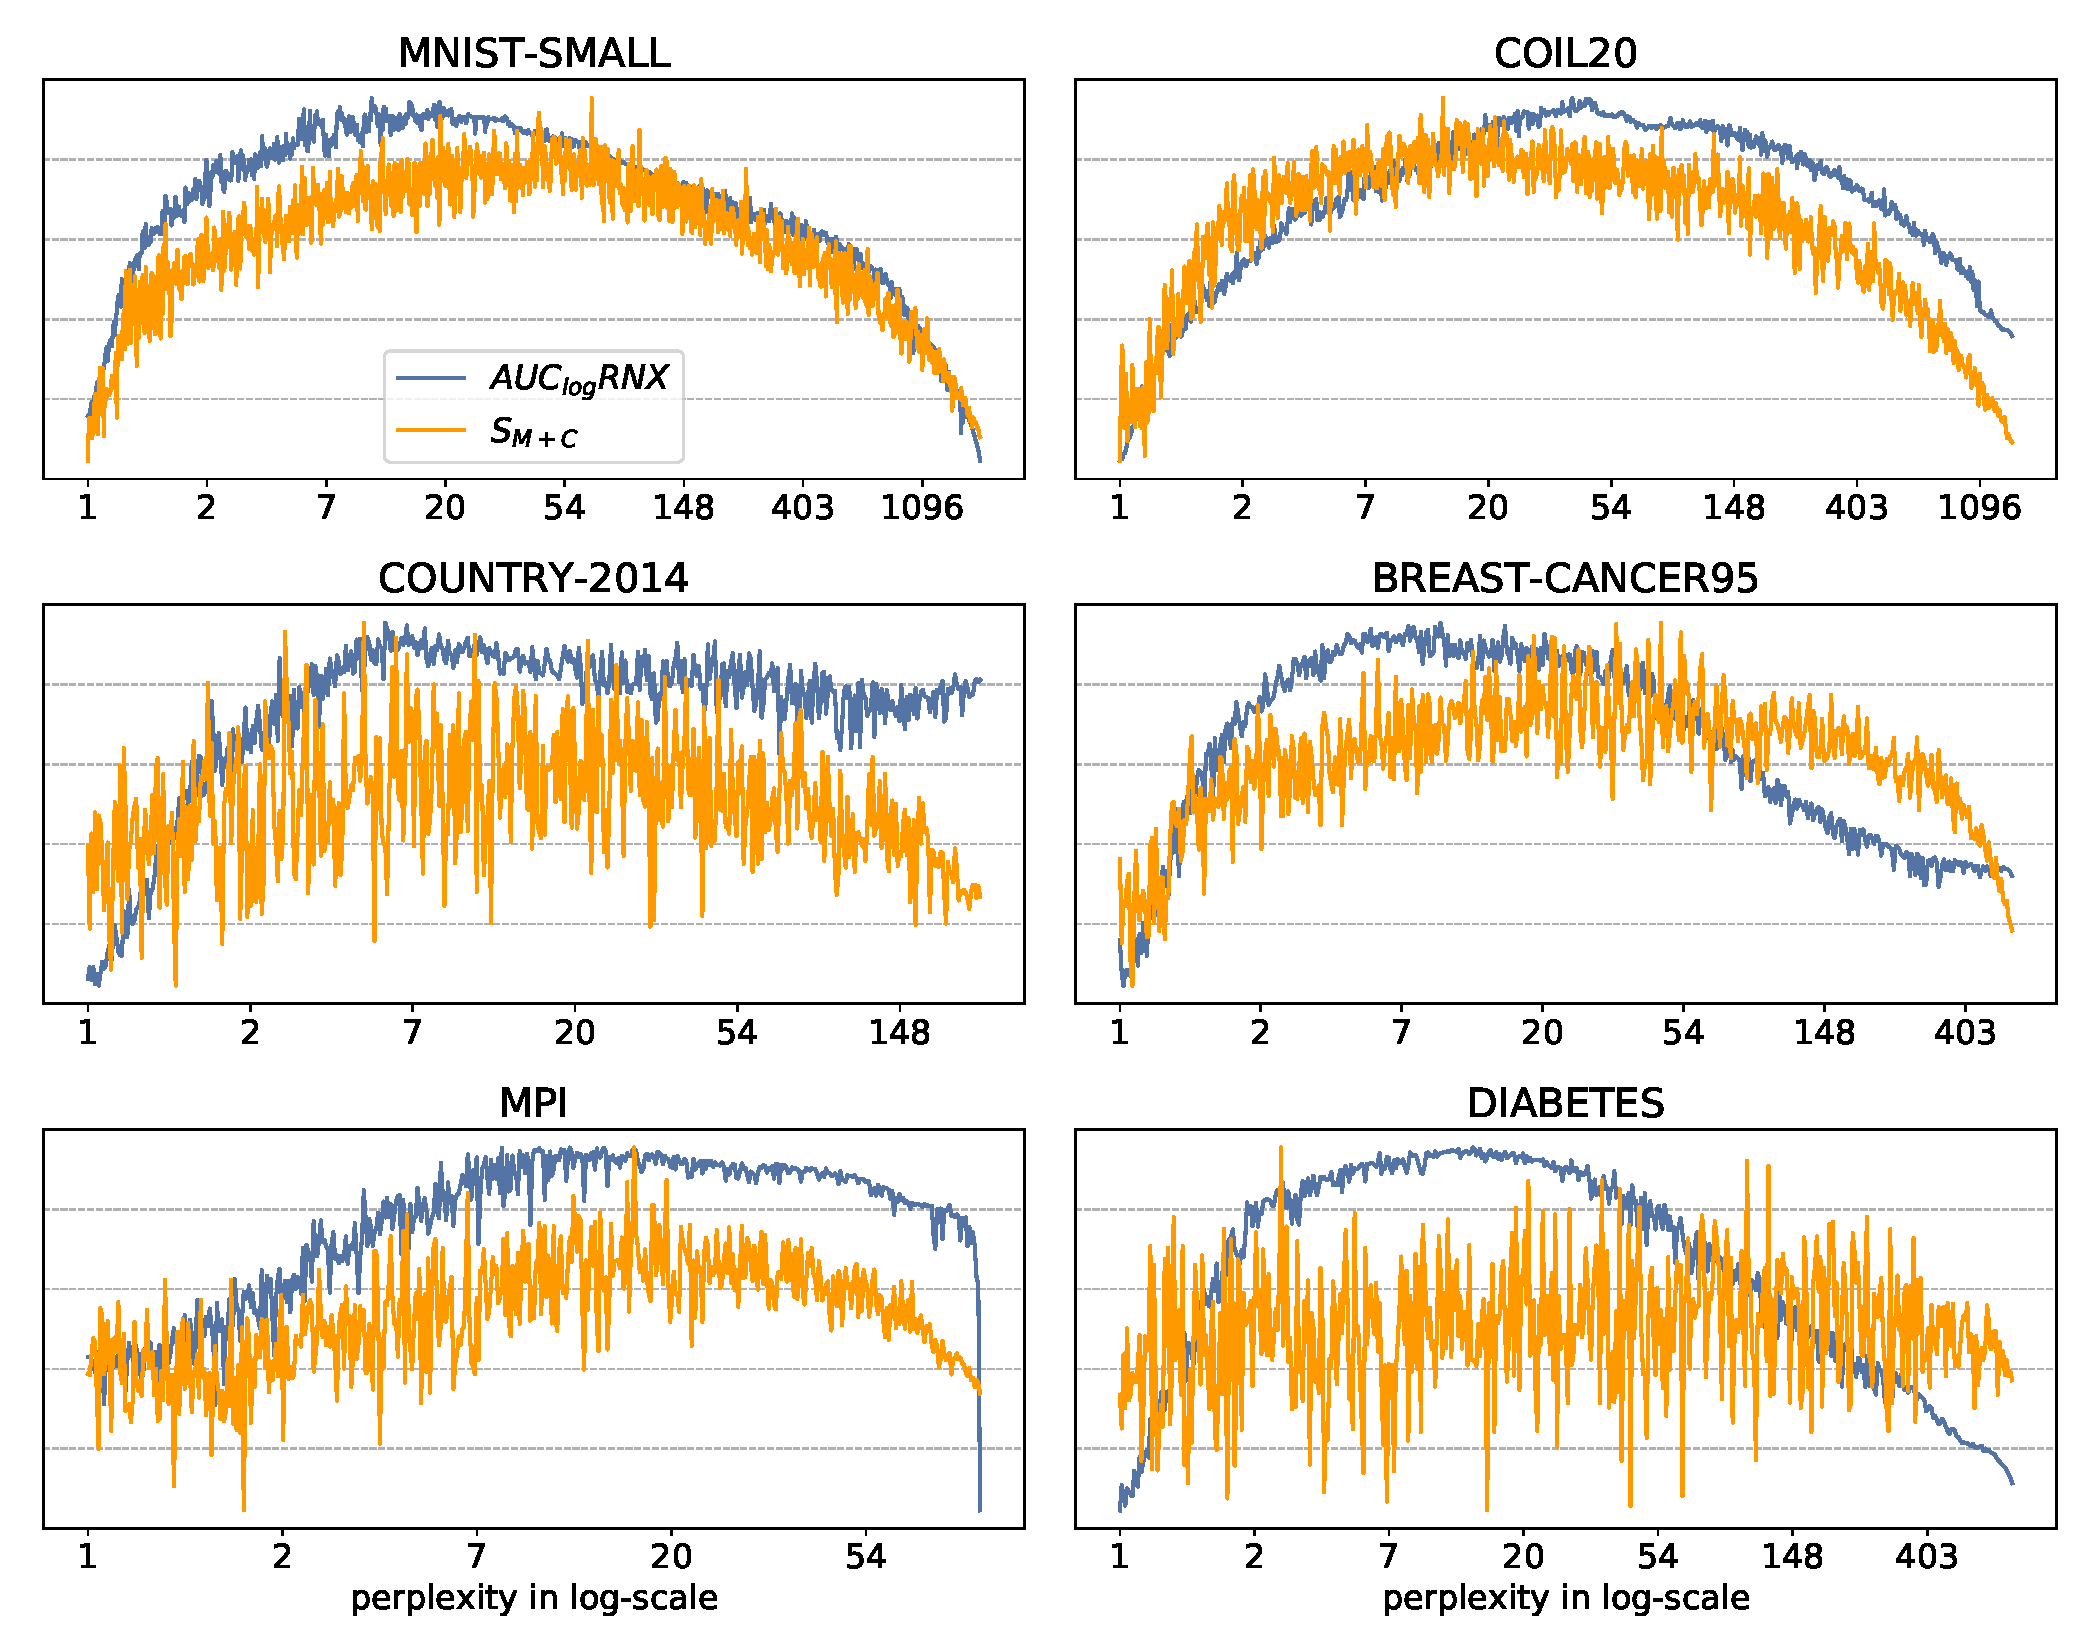
\includegraphics[scale=0.25]{sall_auc_50.pdf}
\caption{ML+CL agrees with AUC\_RNX score.}\label{fig:sall}
\end{figure}

\vspace{8pt} \par
+ Variance / Stability of the score: analyze Fig.~\ref{fig:score_stability} and explain how BayOpt approach can take into account the variance (uncertainty) of the score.

\begin{figure*}
     \centering
     \begin{subfigure}[b]{0.32\textwidth}
         \centering
         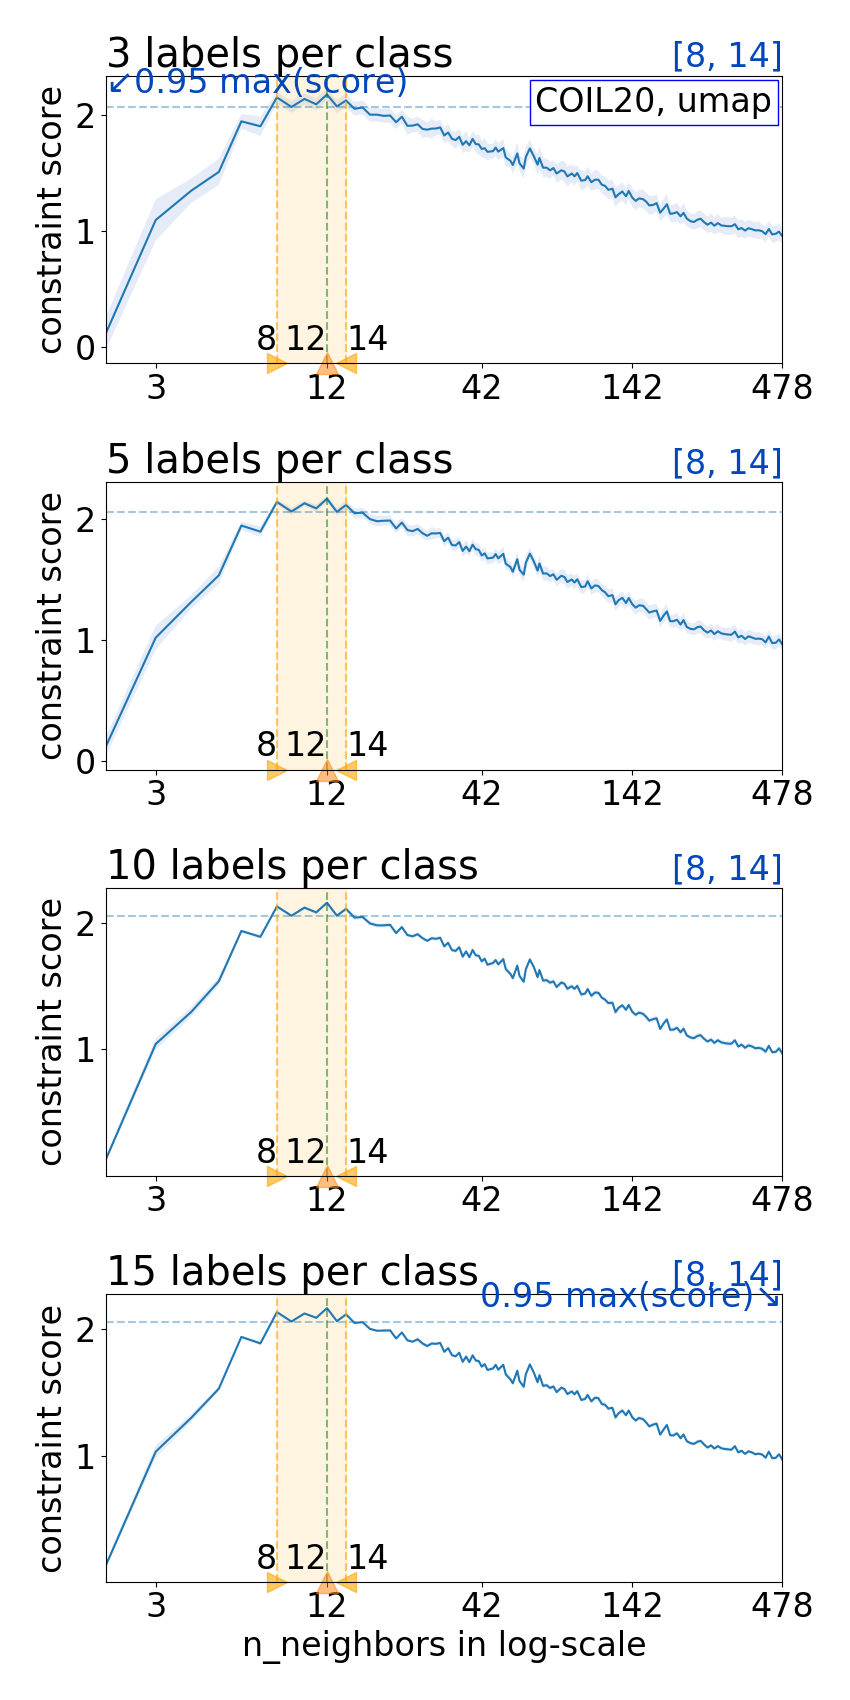
\includegraphics[width=\textwidth]{COIL20_umap_scores}
         \caption{UMAP with COIL20}
         \label{fig:s4}
     \end{subfigure}
     \hfill
     \begin{subfigure}[b]{0.32\textwidth}
         \centering
         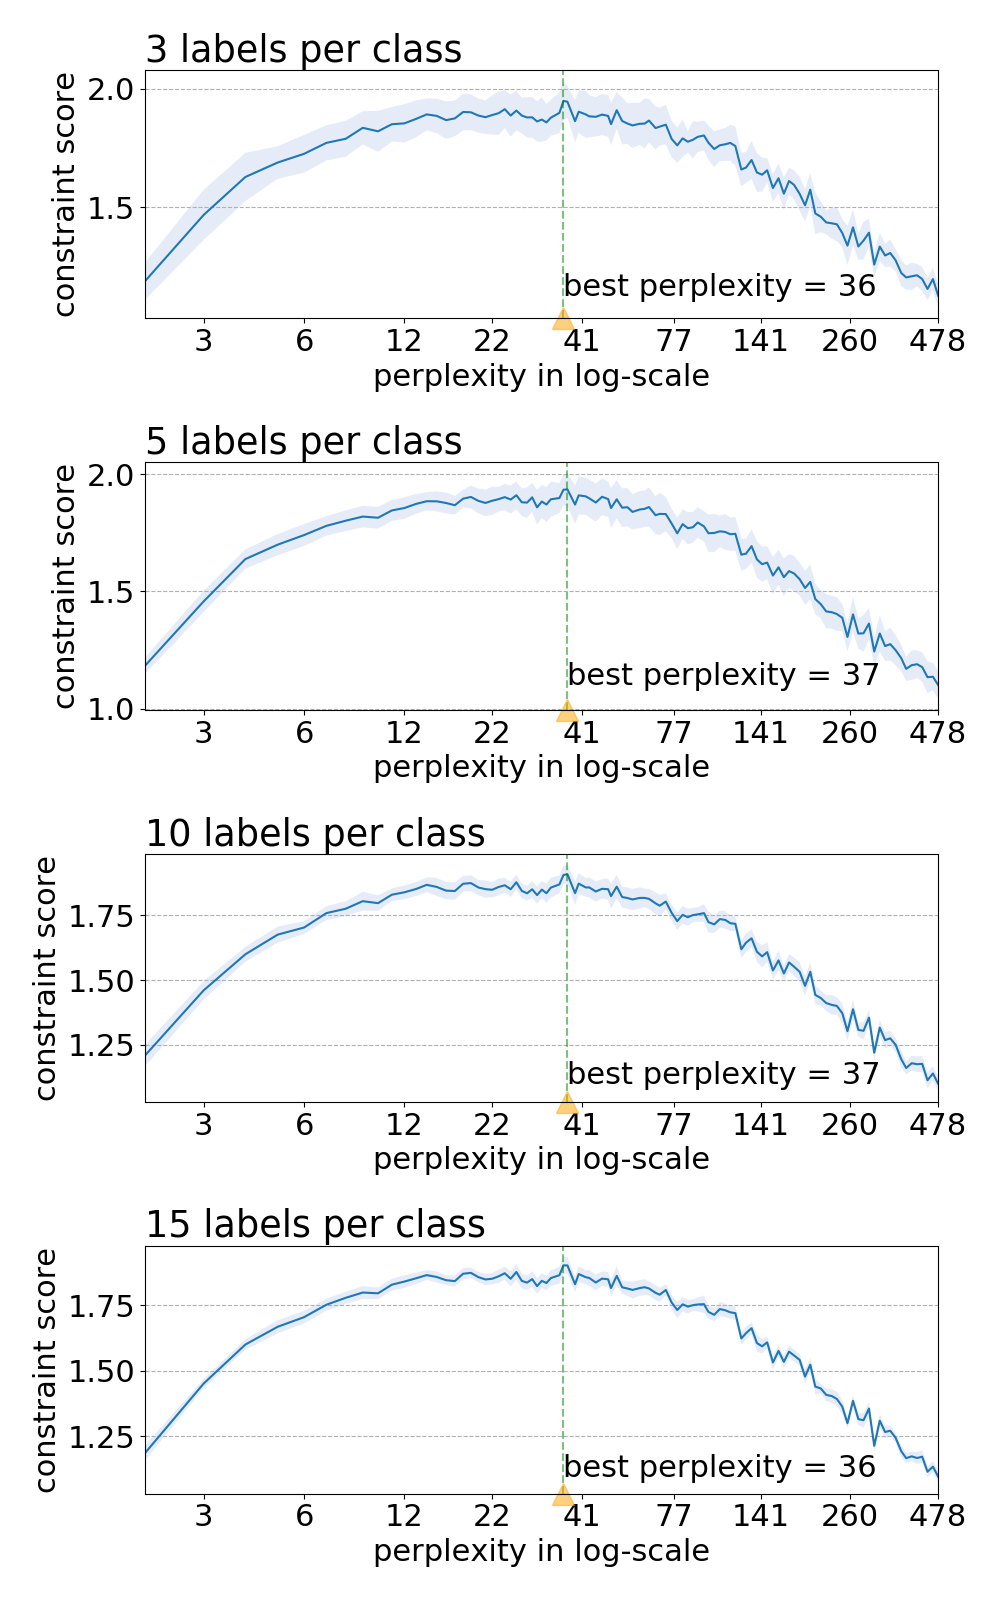
\includegraphics[width=\textwidth]{COIL20_tsne_scores}
         \caption{t-SNE with COIL20}
         \label{fig:s3}
     \end{subfigure}
     \hfill
     \begin{subfigure}[b]{0.32\textwidth}
         \centering
         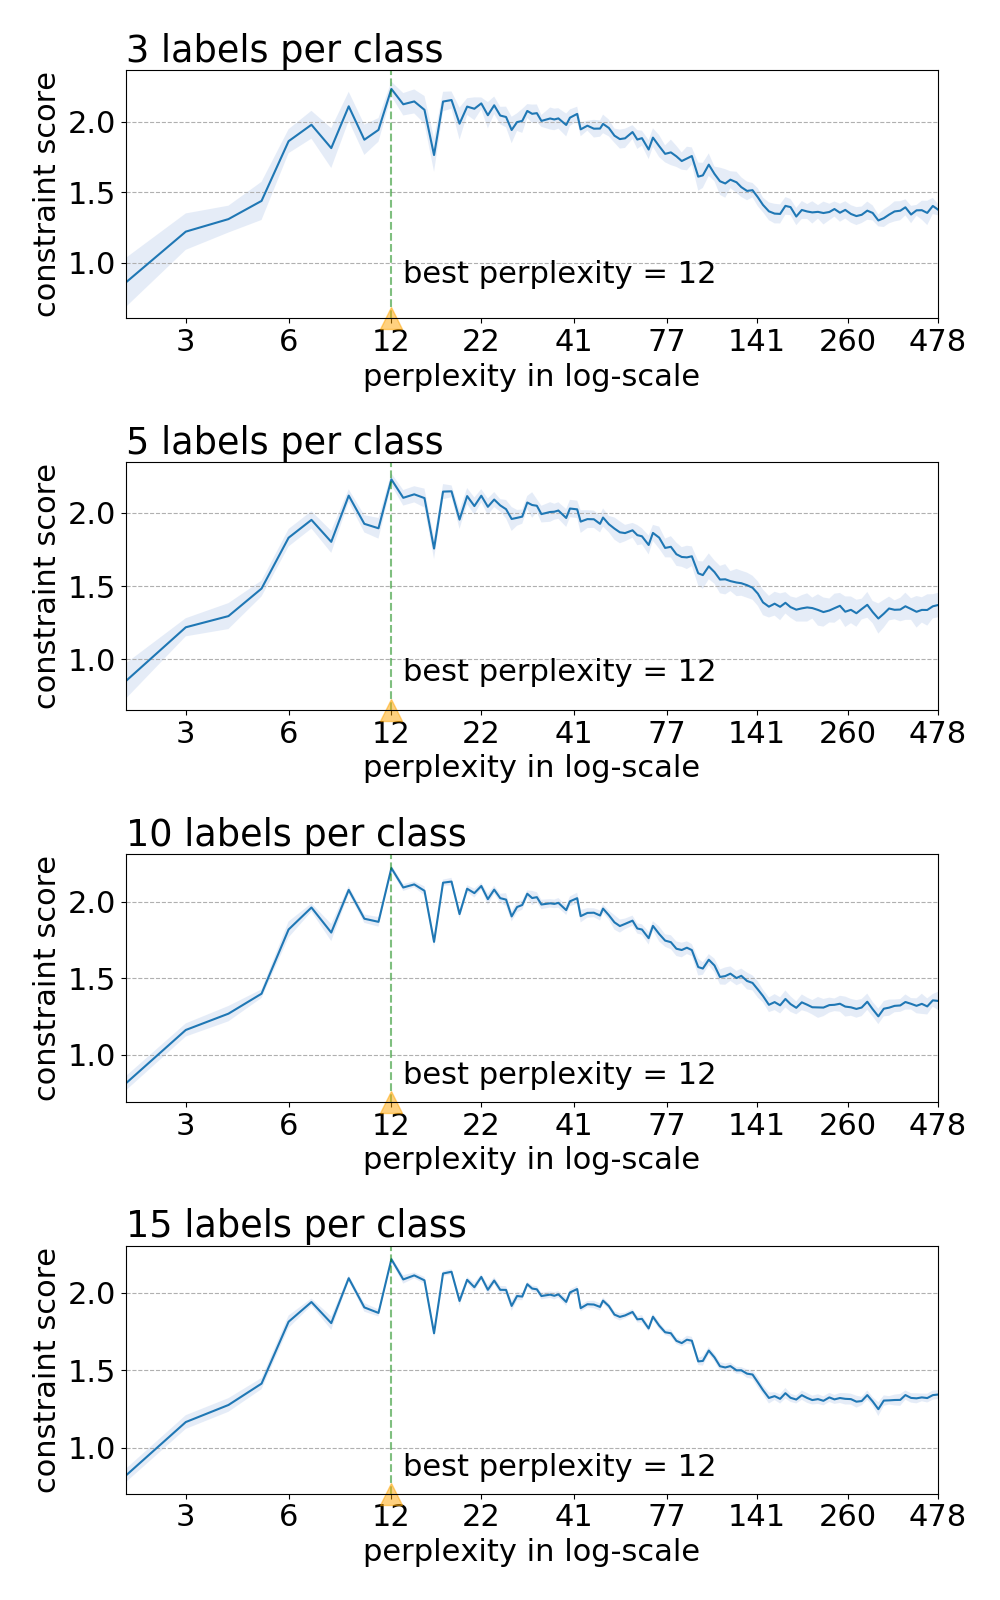
\includegraphics[width=\textwidth]{COIL20_largevis_scores}
         \caption{LargeVis with COIL20}
         \label{fig:s4}
     \end{subfigure}

     \vfill

     \begin{subfigure}[b]{0.32\textwidth}
         \centering
         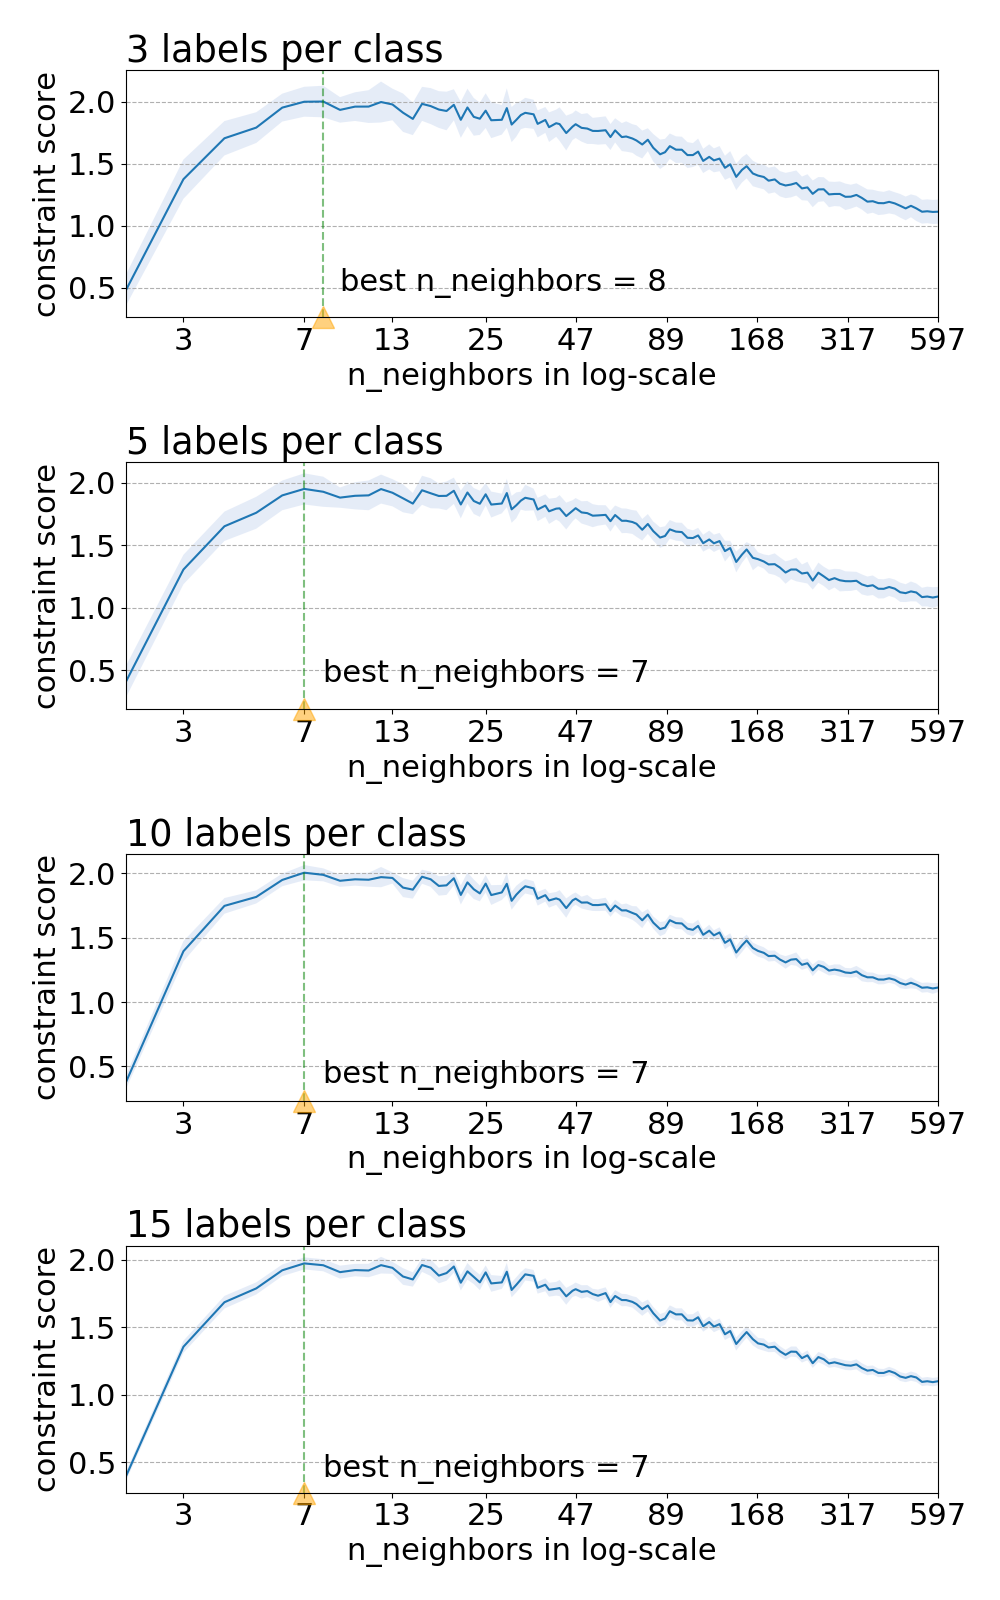
\includegraphics[width=\textwidth]{DIGITS_umap_scores}
         \caption{UMAP with DIGITS}
         \label{fig:s4}
     \end{subfigure}
     \hfill
     \begin{subfigure}[b]{0.32\textwidth}
         \centering
         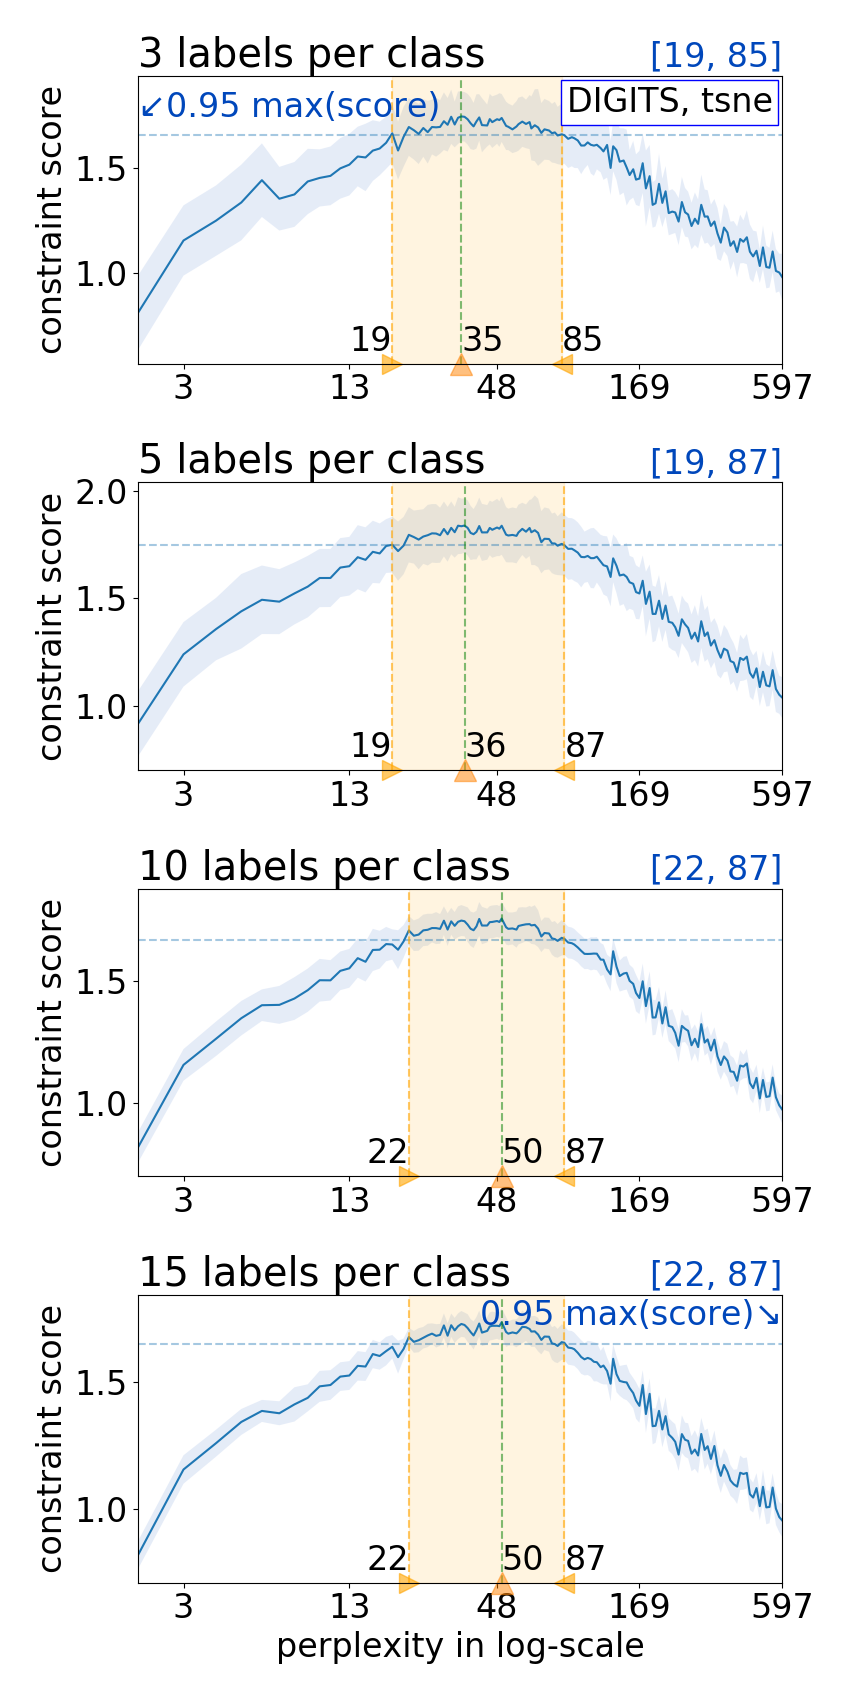
\includegraphics[width=\textwidth]{DIGITS_tsne_scores}
         \caption{t-SNE with DIGITS}
         \label{fig:s3}
     \end{subfigure}
     \hfill
     \begin{subfigure}[b]{0.32\textwidth}
         \centering
         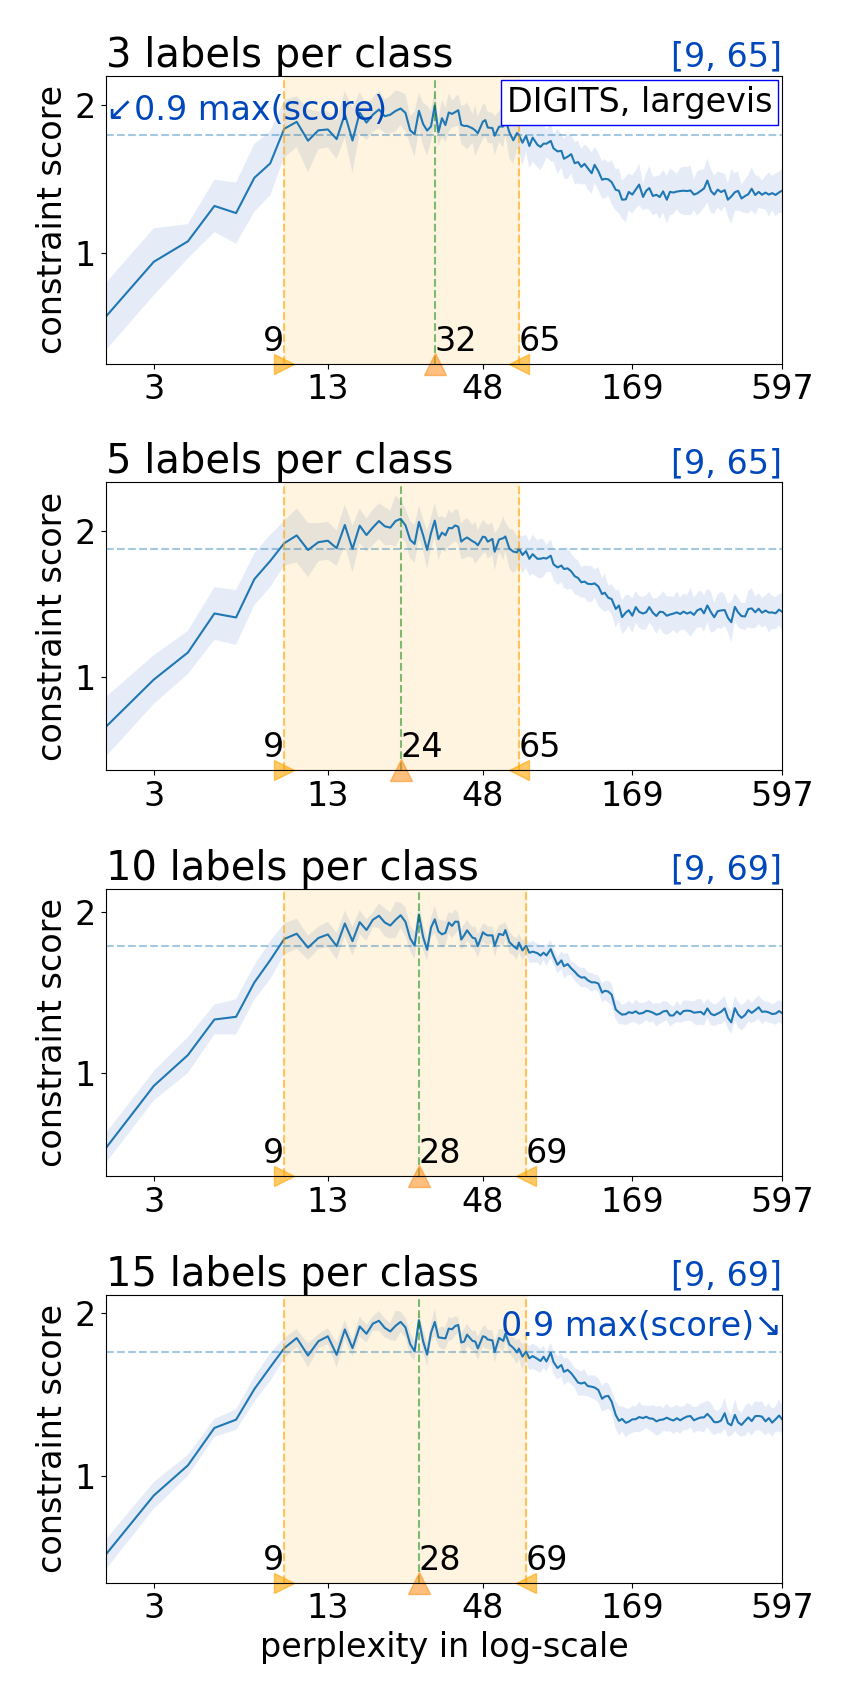
\includegraphics[width=\textwidth]{DIGITS_largevis_scores}
         \caption{LargeVis with DIGITS}
         \label{fig:s4}
     \end{subfigure}

     \caption{Stability of the constraint preserving scores with three methods UMAP, t-SNE and LargeVis for two datasets COIL20 and DIGITS}
     \label{fig:score_stability}
\end{figure*}


\vspace{8pt} \par
To discuss:

+ How to evaluate the visualization corresponding to the optimal hyperparam found by our method? => We can show this optimal viz and other `non-optimal' viz and analyze them visually/intuitively.

+ \st{Compare our score with John's score? (Apply BayOpt to John's metric, compare the predictive score function - the prediction line in the graphs, compare the optimal hyperparameter).}
(John's metric use HD data, time complexity of $O(DN^3)$ while our score is $O(DN^2)$ with a scale factor of the number of constraints.)

+ Compare our result with the method of auto-selecting perplexity of Cao and Wang? (TODO)



%%%%%%%%%%%%%%%%%%%%%%%%%%%%%%%%%%%%%%%%%%%%%%%%%%%%%%%%%%%%%%%%%%%
\section{Discussion}
Meeting 12/07: not sound enough for now, to discuss later.

\par
Discuss the variance of the proposed score (w.r.t to different set of constraints, different number of constraitns).
Say, the constraint-based score is a stochastic function.
Say, how BayOpt can take into account the uncertainty (the variance of the score) to estimate the maximum of this stochastic function.


\par
The violated constraints in our methods correspond to the shortcomming of t-SNE in \cite{wattenberg2016use}.
t-SNE can not preserve the within-cluster distances and between-clusters distances.
[TODO: Add reproduced figures].
The $q_{ij}$-based score can help to understand the defective of the visualization.

\par
Add discussion for UMAP.

\par
Easily generate pairwise constraints from labels.
  Only need small amount of labeled points for each class to generate hundreds of constraints.
  The proposed method only need 200 constraints to work well.
  [TODO: Test with smaller number of constraints to see if it works. 200 constraints seem too much].

\par
Can replace the auto-generated constraints by the manual constraints of the real user.

\par
The user can interact directly in the loop of Bayesian Optimization method to select the next hyperparameter to discover.


\par
Both the constraint-based score and the BayOpt's internal steps are explainable even for the non-technical users. 



%%%%%%%%%%%%%%%%%%%%%%%%%%%%%%%%%%%%%%%%%%%%%%%%%%%%%%%%%%%%%%%%%%%
\section{Conclusion and Future Work}

\par (1) Repeat the problem of hyperparameter tuning for DR methods and our solution:

+ The proposed constraint-based score is indenpendent to how the embedding is produced and can be used with any DR methods.
This score is built upon a limited number of constraints but can distinguish the visualizations prefering local structure and those prefereing global structure.

+ A finding that Bayesian Optimization approach fits well in our problem.


\vspace{8pt}
\par (2) Summary the advantages of the two above elements

+ The constraint-based score agree the the well-known quality metric.

+ This score can be visually represented to explain the violated pairs.

+ By combining this score with BayOpt approach, we can tune many hyperparameters at the same time for many widely used DR methods like t-SNE or UMAP.

+ BayOpt takes into account the uncertainty in the score values and also explainable. We can observe the internal optimization step to anwser the question: why to choose the next promissing hyperparameters to try?


\vspace{8pt}
\par (4) Future work:

(a) User experiment:

+ Integrate the user's feedback in two stages of our workflow.
The users can select the pairwise constraints or label some points (used to generate the constraints) to build the score.
They can also manualy select the next hyperparameters to evaluate in a customized interactive BayOpt framework.

+ Take the preference of the users on the presented visualizations to evaluate the quality of the visualization. We search for if the best visualization selected by the user corresponds to the result of our method.


(b) Integrate directly the pairwise constraints into the optimization process of BayOpt.
BayOpt is now used as a generic toolbox to find the extreme of a blackbox costly objective function.
Our idea is to use the pairwise constraint to modify the kernel in the covariance function of Gaussian Process model, which is the core element of BayOpt.
